% !TeX program = xelatex
\documentclass[12pt,a4paper]{ctexart}
\usepackage[left=2.6cm,right=2.6cm,top=2.6cm,bottom=2.6cm]{geometry}
\usepackage{setspace}
\usepackage{amsmath,amssymb,bm}
\usepackage{booktabs}
\usepackage{array}
\usepackage{longtable}
\usepackage{graphicx}
\usepackage{caption}
\usepackage{hyperref}
\hypersetup{hidelinks}

\setlength{\parindent}{2em}
\setlength{\parskip}{0pt}
\linespread{1.35}
\newcommand{\coverline}[2]{%
  \makebox[3.2cm][s]{#1}：\quad
  \underline{\makebox[7.4cm][c]{#2}}\\[0.42cm]
}
\ctexset{
  section={format=\bfseries\zihao{4},number=\Roman{section}.},
  subsection={format=\bfseries\zihao{-4},number=\Alph{subsection}.}
}

\begin{document}

\begin{titlepage}
\centering
\vspace*{2.3cm}
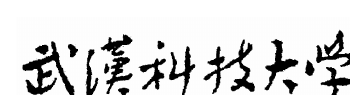
\includegraphics[width=5.2cm]{figures/wust_mark.png}\\[0.8cm]
{\zihao{0}\bfseries 本科毕业论文外文翻译}\\[2.4cm]

\begin{flushleft}
\hspace*{1.0cm}{\zihao{3}\bfseries 外译文题目：}\quad
\underline{\makebox[9.0cm][c]{\zihao{4} 基于 PPO 算法的爬索机器人减振控制}}
\end{flushleft}

\vfill
{\zihao{4}
\coverline{学\hspace{1em}院}{人工智能与自动化学院}
\coverline{专\hspace{1em}业}{机器人工程}
\coverline{学\hspace{1em}号}{202204416388}
\coverline{学生姓名}{杜云帆}
\coverline{指导教师}{陈志环}
\coverline{日\hspace{1em}期}{二〇二六年五月}
}
\vspace*{1.3cm}
\end{titlepage}

\begin{center}
{\zihao{3}\bfseries Vibration Damping Control of Cable-climbing Robots Based on PPO Algorithm}\\[0.5cm]
{\zihao{4}Yangru Zhou, Kaiwei Ma, Fengyu Xu, Tengda Xie}\\
{\zihao{-4}College of Automation and College of Artificial Intelligence,\\
Nanjing University of Posts and Telecommunications, Nanjing, China}\\[1.0cm]
{\zihao{3}\bfseries 基于 PPO 算法的爬索机器人减振控制}\\[0.5cm]
{\zihao{4}周扬茹，马凯威，徐丰煜，谢腾达}\\
{\zihao{-4}南京邮电大学自动化学院、人工智能学院，中国南京}
\end{center}

\section*{摘要}
为解决缆索振动环境下爬索机器人攀爬不稳定的问题，本文提出了一种基于 PPO（Proximal Policy Optimization，近端策略优化）算法的减振控制方法。首先，基于具有变刚度、变阻尼特性的氮气弹簧-磁流变（MR）阻尼器耦合加载机构，建立了 BP 神经网络输出力模型。仿真结果表明，所设计输出力模型的误差控制在 6.6 N 以内，验证了模型的准确性。随后，确定了 PPO 算法下机器人输出的工作空间和状态空间，并设计奖励函数和网络结构，以保证学习过程中能够进行有效探索。最后，在 MATLAB Simulink 中搭建仿真环境。仿真结果表明，当缆索振动频率为 10 Hz、振幅为 4 mm 时，与 PID 控制相比，PPO 算法使机器人的攀爬速度稳定性提升了 31.6\%。

\noindent\textbf{关键词：} 爬索机器人；PPO 算法；变刚度与变阻尼；耦合加载机构；BP 神经网络

\section{引言}
斜拉桥缆索作为承受主要载荷的关键部件，其安全性和稳定性至关重要，因此定期检测与维护不可或缺。目前，爬索机器人已经成为大型桥梁缆索自动化检测的重要工具。在爬索机器人的发展过程中，设计一种新型减振机构及相应控制算法，使机器人能够稳定夹持缆索并平稳运动，是研究人员面临的核心挑战。针对这一问题，国内外学者围绕爬索机器人减振技术开展了大量探索与研究，其方法大致可分为三类：弹簧储能减振方法\,[1,2]、机械夹紧减振方法\,[3,4]和仿生包络夹持减振方法\,[5,6]。

采用弹簧储能夹持方式的爬索机器人结构简单、运动效率高，并具有较好的承载能力和越障能力。然而，由于缆索通常处于动态环境中，弹簧夹持机构的稳定性容易受到风载和结构振动影响，从而导致机器人滚轮发生打滑。机械夹紧和仿生包络夹持方法虽然能够更牢固地抱紧缆索，但实现结构复杂、攀爬速度较慢，不适合高效率攀爬。因此，研究人员开始利用磁流变阻尼器连续可调的阻尼力来提升系统稳定性，并减小外部风扰对系统的影响。

磁流变阻尼器是一类利用磁流变效应的新型智能阻尼装置，能够较好地与控制系统集成，并具有较高可靠性。在建模方面，Bai 等\,[7]提出了基于电阻-电容算子的磁流变阻尼器滞回模型；Lu 等\,[8]提出了基于 sigmoid 函数的磁流变动力学模型，用于实时控制系统；Liu 等\,[9]设计了座椅悬架磁流变阻尼器，并提出了基于改进 IFOA 算法的磁流变阻尼器动力学模型。在控制方面，Gao 等\,[10]提出了基于 Lyapunov 方程的自适应最优容错控制算法，显著提高了车辆悬架减振效果；Yoon 等\,[11]提出了应用于磁流变阻尼器的滑模控制器，实现了悬架系统振动控制；Kumar 等\,[12]针对船舶推进系统中的磁流变阻尼器系统设计了自适应神经模糊推理系统，降低了扭转和横向振动；Lei 等\,[13]提出了模糊 PID 算法，并在振动试验平台上验证了磁流变阻尼器的减振效果，表明模糊 PID 算法能够有效抑制磁流变阻尼器中的微振动。上述控制策略均在不同程度上改善了减振效果。然而，由于磁流变阻尼器具有显著非线性，上述算法难以实现精确控制。

强化学习在解决未知模型复杂线性系统的最优控制问题中发挥着重要作用。将强化学习与控制理论结合，可以形成自适应动态规划理论的基础，这是一类具有学习能力和优化能力的数据驱动智能控制算法，在鲁棒控制、最优控制和自适应控制等方向已有较多理论成果。Hao 等\,[14]提出了一种结合强化学习和虚拟模型控制的四足机器人分层控制框架，实现了带规划步态的高效率运动。Zhang 等\,[15]使用改进 Q-Learning 强化学习算法，提高了蛇形机器人在多障碍路径中的运动平滑性和适应能力。Qin 等\,[16]采用 DDPG 算法，在推进器故障导致跟踪性能低于预设阈值时生成补偿控制信号，从而实现后续容错控制。Amar 等\,[17]提出了基于 TRPO 算法的微机器人智能自主精确导航控制系统，使盘形磁性微机器人能够在真实环境中学习通向随机目标位置的最优路径。

尽管强化学习算法已在非线性控制领域取得了成功，但其在爬索机器人中的研究仍较少。因此，本文将氮气弹簧-磁流变阻尼器耦合加载机构应用于爬索机器人，建立耦合加载机构的输出力模型，并进一步采用 PPO 强化学习算法控制爬索机器人，以提升缆索检测机器人在振动环境下的攀爬稳定性。

\section{耦合加载机构输出力建模}
当缆索发生剧烈振动时，机器人滚轮与缆索表面之间的摩擦力不足，容易导致机器人打滑，进而引起机器人加速度变化和攀爬不稳定\,[18]。该摩擦力由机器人加载机构的夹持力提供。因此，有必要设计一种新型变刚度、变阻尼耦合加载机构，用于替代原有弹簧加载机构。该新机构能够根据缆索振动情况灵活调节加载力，以满足机器人稳定攀爬的要求。

\begin{figure}[htbp]
\centering
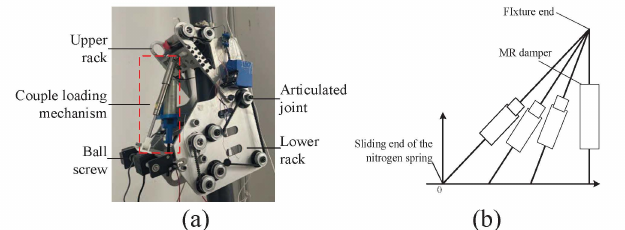
\includegraphics[width=0.86\textwidth]{figures/fig1.png}
\caption{氮气弹簧-MR 阻尼器耦合加载机构。（a）耦合加载机构安装示意图；（b）氮气弹簧倾角示意图。}
\end{figure}

新型耦合加载机构的整体结构如图1（a）所示。该加载机构由 MR 阻尼器与氮气弹簧耦合而成，用于替代原有单一普通螺旋弹簧。该结构能够为机器人提供可调、可控的阻尼力以夹紧缆索，从而提升攀爬稳定性。氮气弹簧变刚度原理如图1（b）所示。氮气弹簧通过改变支撑角快速调节悬架刚度；MR 阻尼器通过改变输入电流调节内部磁场强度，进而改变加载机构的刚度和阻尼，调节输出加载力，提高机器人攀爬稳定性。

由于 MR 阻尼器存在复杂的非线性滞回现象，非参数模型相比参数模型具有更强的非线性建模能力、更好的适应性、更广的适用性、数据驱动特征和鲁棒性。因此，本文采用单隐层 BP 神经网络构建氮气弹簧-MR 阻尼器耦合加载机构的输出力模型。网络结构如图2所示。

\begin{figure}[htbp]
\centering
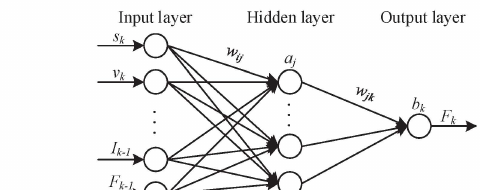
\includegraphics[width=0.72\textwidth]{figures/fig2.png}
\caption{BP 神经网络结构。}
\end{figure}

氮气弹簧-MR 阻尼器耦合加载机构的性能与前一时刻状态有关\,[19]。因此，模型输入选取当前位移 $s_k$、速度 $v_k$、输入电流 $I_k$、氮气弹簧角度 $\beta_k$，以及上一时刻位移 $s_{k-1}$、速度 $v_{k-1}$、输入电流 $I_{k-1}$、角度 $\beta_{k-1}$ 和阻尼力 $F_{k-1}$；模型输出为当前阻尼力 $F_k$。其中，$a_i$ 和 $b_k$ 分别为 BP 神经网络隐含层和输出层神经元阈值，$w_{ij}$ 和 $w_{jk}$ 分别为输入层到隐含层、隐含层到输出层之间的连接权值。

由此，神经网络输出力模型具有 9 个输入神经元和 1 个输出神经元。隐含层节点数可根据输入、输出节点数计算。隐含层节点数 $q$ 通常采用下式确定：
\begin{equation}
q=\sqrt{m'+n'}+c ,
\end{equation}
其中，$m'$ 表示输入层节点数，$n'$ 表示输出层节点数，$c$ 为 1 到 10 之间的整数。因此，隐含层节点数范围确定为 4 到 13。将 BP 网络依次设置为上述 10 种隐含层节点数，并计算训练集均方误差（MSE），最小误差对应的节点数即为最优隐含层节点数。本文最终将隐含层节点数设置为 12。

\begin{figure}[htbp]
\centering
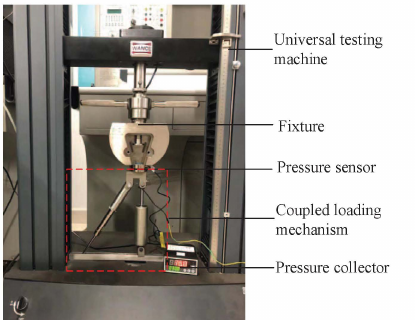
\includegraphics[width=0.62\textwidth]{figures/fig3.png}
\caption{耦合加载机构测试平台。}
\end{figure}

采用万能试验机对氮气弹簧-MR 阻尼器耦合加载机构进行样本采集，测试平台如图3所示。选择正弦信号作为阻尼器活塞输入位移，振幅 $A_0$ 分别为 2 mm 和 5 mm，频率 $f$ 分别为 1 Hz 和 5 Hz，输入电流 $I$ 范围为 0 到 2 A，氮气弹簧角度 $\beta$ 范围为 $37^\circ$ 到 $61^\circ$，采样时间为 10 s。共采集 5000 组数据，其中 3000 组用于训练，1000 组用于验证，1000 组用于测试，以验证模型有效性。

在训练 BP 神经网络模型前，需要对数据进行归一化。本文采用均值-方差方法，使数据缩放能够体现均值和方差影响下的动态关系：
\begin{equation}
W'=\frac{W-W_{\mathrm{mean}}}{W_{\mathrm{var}}},
\end{equation}
其中，$W_{\mathrm{mean}}$ 表示数据均值，$W_{\mathrm{var}}$ 表示数据方差。

在 BP 神经网络中，从输入层到隐含层的激活函数设置为 tan-sigmoid 函数，从隐含层到输出层的激活函数设置为 purelin 函数。采用均方误差（MSE）函数作为性能指标分析误差，理想 MSE 为 0.00005。MSE 函数为：
\begin{equation}
\mathrm{MSE}=\frac{1}{N}\sum_{i=1}^{N}\left(F_i-\hat{F}_i\right)^2,
\end{equation}
其中，$F_i$ 表示第 $i$ 个样本的真实输出力，$\hat{F}_i$ 表示模型对第 $i$ 个样本的预测值，$N$ 表示样本数量。

神经网络迭代过程如图4所示。经过 316 次迭代后，模型达到最优均方误差 0.000045912。

\begin{figure}[htbp]
\centering
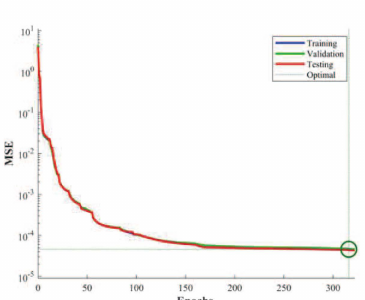
\includegraphics[width=0.64\textwidth]{figures/fig4.png}
\caption{BP 神经网络迭代过程。}
\end{figure}

\begin{figure}[htbp]
\centering
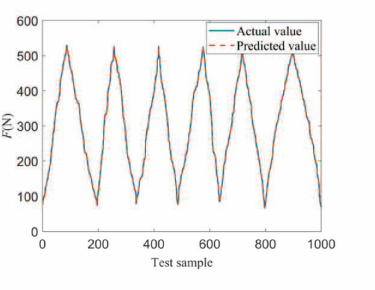
\includegraphics[width=0.64\textwidth]{figures/fig5.png}
\caption{预测阻尼力与真实阻尼力对比。}
\end{figure}

\begin{figure}[htbp]
\centering
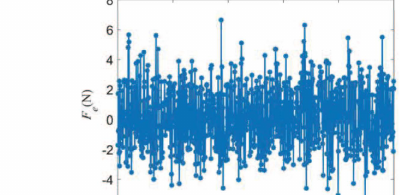
\includegraphics[width=0.58\textwidth]{figures/fig6.png}
\caption{预测阻尼力与真实值之间的误差。}
\end{figure}

由图5和图6可观察到阻尼力 $F$ 的预测值与真实值对比曲线，以及误差曲线 $F_e$。可以看出，所设计的神经网络阻尼力输出模型具有良好的拟合性能，预测值整体接近真实值，二者误差控制在 6.6 N 以内，说明所建立模型具有正确性。

\section{PPO 减振算法设计}
PPO 算法即近端策略优化算法，是一种基于策略梯度的更新优化算法。对于配备氮气弹簧-MR 阻尼器耦合加载机构的爬索机器人系统，PPO 算法能够在连续动作空间任务中取得较好控制效果。

\subsection{PPO 算法}
PPO 采用 Actor-Critic 网络结构输出连续空间动作，并利用历史数据多次更新旧动作网络策略参数。该算法通过 Actor 网络拟合行为策略，通过 Critic 网络拟合价值函数。行为策略可表示为
\begin{equation}
\pi_\theta(a_t|s_t)=P(s_t,a_t),
\end{equation}
其中，$\pi_\theta$ 表示当前策略，$\theta$ 为动作网络中可更新的参数，$t$ 为时间，$s_t$ 和 $a_t$ 分别表示 $t$ 时刻的状态和动作，$P(s_t,a_t)$ 表示在当前策略下、状态 $s_t$ 中采取动作 $a_t$ 的概率。

价值函数可描述为：
\begin{equation}
V(s_t,a_t)=E\left[r_t+\gamma V(s_{t+1},a_{t+1})\right],
\end{equation}
其中，$V(s_t,a_t)$ 表示在状态 $s_t$ 下采取动作 $a_t$ 的估计价值函数，$r_t$ 表示获得的奖励，$\gamma$ 为折扣因子，用于平衡当前估计价值和未来估计价值的权重，$V(s_{t+1},a_{t+1})$ 表示在下一状态 $s_{t+1}$ 下采取动作 $a_{t+1}$ 的估计价值函数，$E$ 表示期望估计值。

Actor 网络和 Critic 网络的梯度更新通过估计优势函数实现：
\begin{equation}
A(s_t,a_t)=\sum_{t'=t}^{n}\gamma^{t'-t}r_{t'}-V(s_t,a_t),
\end{equation}
其中，$A(s_t,a_t)$ 表示 $t$ 时刻的优势函数，$n$ 表示一个回合中的总步数，$t'$ 表示从 $t$ 时刻到总步数 $n$ 之间的某一时刻。

PPO 采用重要性采样方法提高数据利用效率。其思想是为每个数据点分配一个权重，该权重表示目标策略与行为策略之间的比值，从而在不影响策略梯度正确性的前提下提高数据利用效率。因此，历史数据可用于更新新策略。更新完成后，将新策略参数复制给旧策略。

Actor 网络更新可描述为：
\begin{equation}
k(\theta,\theta')=\frac{\pi_\theta(s_t,a_t)}{\pi_{\theta'}(s_t,a_t)},
\end{equation}
\begin{equation}
J(\theta)=\min\left\{
k(\theta,\theta')A_{\theta'},
\mathrm{clip}\left[k(\theta,\theta'),1-\epsilon,1+\epsilon\right]A_{\theta'}
\right\},
\end{equation}
其中，$\pi_{\theta'}$ 表示旧策略，$A_{\theta'}$ 表示由旧策略得到的优势函数，$k(\theta,\theta')$ 表示新旧策略之间的差异，$\epsilon$ 为裁剪因子，用于限制新旧策略之间的差异，$\mathrm{clip}$ 为裁剪函数，将 $k(\theta,\theta')$ 的值限制在 $1-\epsilon$ 到 $1+\epsilon$ 之间，$J(\theta)$ 为 Actor 网络目标函数。

Critic 网络通过最小化损失函数进行更新。损失函数为：
\begin{equation}
L=\frac{1}{N}\sum
\left[
V(s_t,a_t)-E\left(\sum_{t'=t}^{n}\gamma^{t'-t}r_{t'}\right)
\right]^2 ,
\end{equation}
其中，$L$ 表示损失函数，$N$ 表示历史交互数据集中的样本数量。

\subsection{马尔可夫决策过程的形式化定义}
本文将爬索机器人攀爬不稳定问题建模为马尔可夫决策过程（MDP），并利用 PPO 算法训练氮气弹簧-MR 阻尼器耦合加载机构控制器。MDP 形式化包括网络框架设计、状态表示、动作表示和奖励函数设计。

\begin{figure}[htbp]
\centering
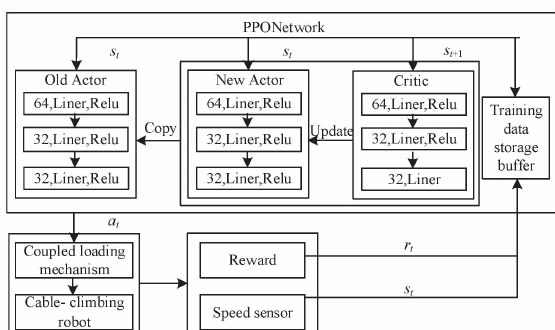
\includegraphics[width=0.86\textwidth]{figures/fig7.png}
\caption{训练网络框架。PPO 网络包括 Old Actor、New Actor 和 Critic，并通过奖励、速度传感器、耦合加载机构及爬索机器人环境形成闭环训练。}
\end{figure}

文中 PPO 网络对 Actor 和 Critic 均采用带 ReLU 激活的 Linear 全连接层（图7）。Critic 网络最后一层首先采用 Linear 层，以加快训练早期价值函数拟合。Actor 输出用于调节电流 $I$ 和氮气弹簧角度 $\beta$，进而控制阻尼力 $F$，影响机器人加速度。在训练过程中，通过观测速度值计算相应奖励并存入缓冲区。当缓冲区数据量达到要求后，更新 New Actor 和 Critic 网络梯度，然后清空缓冲区，并将 New Actor 策略参数复制到 Old Actor。

在状态表示方面，综合考虑机器人运动状态、智能体处理效率和环境等因素，选择五元组 $(v_l, v_e, I_{v_e}, I, \beta)$ 作为观测状态信息。其中，$v_e=0.15-v_l$ 使机器人能够感知当前速度与目标速度之间的差值，并根据误差大小调整速度控制策略；$I_{v_e}$ 有助于机器人累积历史误差，并考虑历史误差对速度控制的影响，从而更快消除稳态误差，提高控制精度和稳定性。

MR 阻尼器阻尼调节需要实时调制磁场强度和方向。因此，本文采用连续动作空间控制爬索机器人上升。控制动作由 MR 阻尼器电流 $I$ 和氮气弹簧角度 $\beta$ 组成的二维动作空间构成。为防止机器人对缆索夹持过松或过紧，导致打滑或夹持过度，连续动作空间定义为：
\begin{equation}
A=\{(I,\beta)\mid 0\le I\le 2,\;37\le \beta\le 61\}.
\end{equation}

奖励函数设计直接影响动作选择。为保证训练稳定高效，本文根据观测状态值构造加权奖励 $r_t$。$r_t$ 由速度误差奖励和误差变化奖励组成，目标是驱动机器人速度误差趋近于零。所有奖励值均为负值，以鼓励策略减少完成任务所需步数。奖励函数可描述为：
\begin{equation}
r_t=-(k_1v_e+k_2e_c),
\end{equation}
其中，$k_1$ 和 $k_2$ 为权重系数，$e_c$ 表示与误差变化相关的控制指标。

综上，PPO 算法伪代码如表1所示。

\begin{longtable}{p{0.95\textwidth}}
\caption{PPO 算法伪代码}\\
\toprule
1. 初始化 Actor 网络和 Critic 网络；\\
2. 初始化经验回放缓冲区 $D$；\\
3. 设置超参数；\\
4. 对每次迭代执行：\\
5. \quad 对每个时间步 $t$ 执行：\\
6. \quad\quad 根据 Actor 网络当前策略 $\pi_\theta$ 选择动作 $a_t$；\\
7. \quad\quad 执行动作 $a_t$，观测奖励 $r_t$ 和新状态 $s_{t+1}$；\\
8. \quad\quad 将经验 $\{s_t,a_t,r_t,s_{t+1}\}$ 存入回放缓冲区 $D$；\\
9. \quad\quad 若 $s_{t+1}$ 为终止状态，则跳出内层循环；\\
10. \quad 结束时间步循环；\\
11. \quad 对多个小批量数据执行：\\
12. \quad\quad 计算优势函数 $A(s_t,a_t)$；\\
13. \quad\quad 计算新旧策略比值 $k(\theta,\theta')$；\\
14. \quad\quad 更新 Actor 网络参数 $\theta$；\\
15. \quad\quad 计算损失并更新 Critic 网络；\\
16. \quad 结束小批量循环；\\
17. \quad 更新旧策略参数 $\theta'$；\\
18. 结束迭代。\\
\bottomrule
\end{longtable}

\section{仿真实验与结果分析}
为验证所提出算法的有效性，本文在 MATLAB Simulink 平台上建立了氮气弹簧-MR 阻尼器神经网络模型，并结合机器人-斜拉索耦合动力学模型\,[18]，在该仿真环境中开展算法训练和仿真实验。

\subsection{训练结果}
在 PPO 训练过程中，训练轮数设置为 2000，每轮最大步数为 600。Actor 和 Critic 学习率均设置为 0.0005。奖励函数折扣因子设置为 0.99，优势函数折扣因子设置为 0.96，裁剪因子设置为 0.2，数据缓冲区大小设置为 4000。奖励函数权重 $k_1$ 和 $k_2$ 分别设置为 3000 和 2500。

损失函数和奖励曲线变化趋势如图8和图9所示。由图8可知，训练初期损失值约为 20，这是由于广义优势函数固有偏差造成的。随着训练轮数增加，损失值在约第 200 轮下降到 1 以下，损失函数曲线逐渐稳定，表明算法已收敛到较优解。这说明 Critic 网络能够快速调整参数以适应优势函数估计中的偏差。

由图9可知，每轮获得的奖励随训练轮数增加而增加。初始阶段奖励约为 -1400，这是因为智能体尚未采取有效动作或策略。随着训练进行，智能体逐渐输出有效动作并采用更优策略，到第 1500 轮左右奖励达到约 -60。训练过程中曲线波动也持续减小。

\begin{figure}[htbp]
\centering
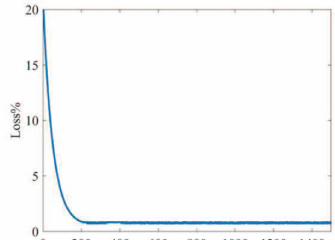
\includegraphics[width=0.58\textwidth]{figures/fig8.png}
\caption{损失函数变化趋势。}
\end{figure}

\begin{figure}[htbp]
\centering
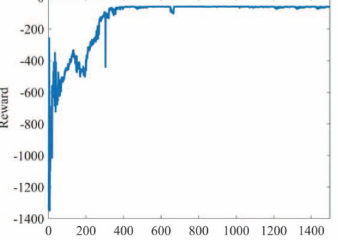
\includegraphics[width=0.58\textwidth]{figures/fig9.png}
\caption{奖励函数变化趋势。}
\end{figure}

\subsection{仿真结果与分析}
为模拟缆索振动激励，采用正弦扰动，频率设置为 1 Hz 和 10 Hz，振幅设置为 2 mm 和 4 mm，从而形成四组正弦激励信号。采用 PPO 强化学习算法对系统进行训练和控制，并将传统 PID 控制作为仿真对照组。PID 参数依据速度误差 $v_e$ 和加速度误差 $e_c$ 调节，经过反复整定后设定为 $K_p=7$、$K_i=4$、$K_d=0.2$。两种控制方法下机器人攀爬速度曲线如图10所示。

\begin{figure}[htbp]
\centering
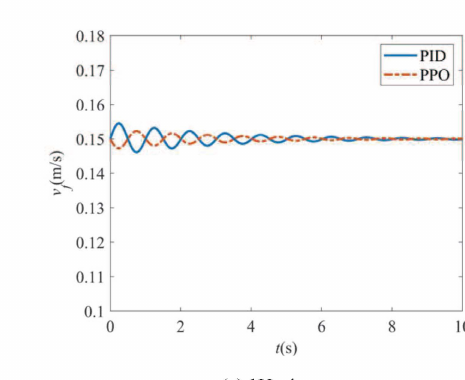
\includegraphics[width=0.48\textwidth]{figures/fig10a.png}
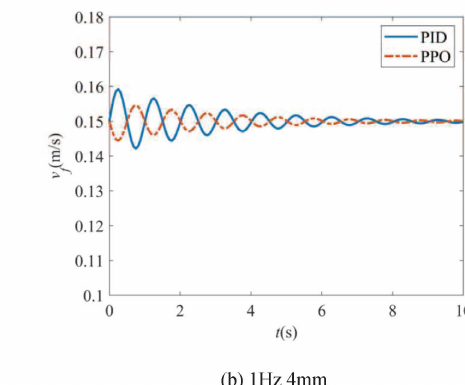
\includegraphics[width=0.48\textwidth]{figures/fig10b.png}\\[0.3em]
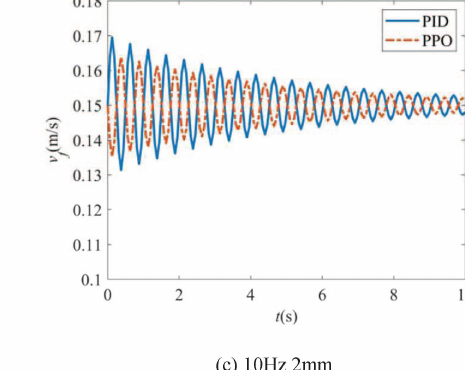
\includegraphics[width=0.48\textwidth]{figures/fig10c.png}
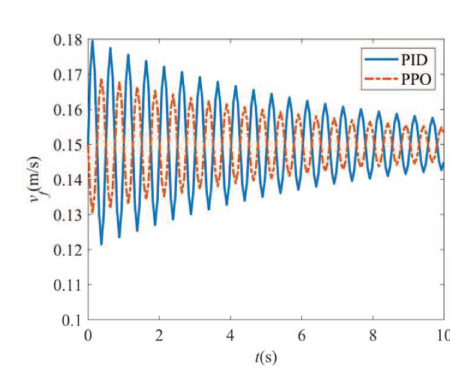
\includegraphics[width=0.48\textwidth]{figures/fig10d.png}
\caption{机器人攀爬速度变化曲线。（a）1 Hz、2 mm；（b）1 Hz、4 mm；（c）10 Hz、2 mm；（d）10 Hz、4 mm。}
\end{figure}

由图10可知，缆索振动频率和振幅增大，会导致爬索机器人攀爬速度波动加剧。当振动频率由 1 Hz 增加到 10 Hz 时，机器人速度波动频率也随之增加。不过，两种控制方法均能将机器人速度调节到约 0.15 m/s 附近。

当振动频率为 1 Hz、振幅为 2 mm 时，PPO 和 PID 两种控制方法均表现良好，但 PPO 算法控制效果更好，速度波动范围仅为 0.008 m/s。当振幅增加到 4 mm 时，速度波动范围略微增大至 0.011 m/s。当振动频率为 10 Hz、振幅为 2 mm 时，PID 控制下速度波动范围为 0.038 m/s，而 PPO 算法下为 0.029 m/s。当振幅增加到 4 mm 时，PID 控制下速度波动范围为 0.057 m/s，而 PPO 算法下为 0.039 m/s。这表明 PPO 算法使速度稳定性提升了 31.6\%。结果说明，与 PID 算法相比，PPO 算法能够提高机器人攀爬速度稳定性，并更有效地抑制振动，证明了 PPO 算法的优越性。

\section{结论}
针对振动条件下爬索机器人攀爬速度不稳定的问题，本文基于氮气弹簧-MR 阻尼器变刚度、变阻尼耦合加载机构，采用 BP 神经网络构建了非参数输出力模型。随后设计了 PPO 强化学习算法。基于 Actor-Critic 原理，构建了算法网络结构，设计了 Actor 和 Critic 网络策略及评价价值函数，设置了速度控制任务的动作空间和状态空间，并设计了奖励函数。通过训练 PPO 算法控制氮气弹簧角度和 MR 阻尼器输入电流，实现对机器人加速度的控制。仿真结果证明了所设计算法的有效性。

然而，该方法仍存在一些不足，例如学习时间较长，需要进一步优化和改进。未来工作将探索如何缩短 PPO 算法训练时间。一种方法是优化神经网络参数，以获得更好的学习效果和更快的收敛速度；另一种方法是采用更高效的深度强化学习算法替代当前算法，从而缩短学习时间。

\section*{参考文献}
\begin{enumerate}
\item X. Li, C. Gao, Y. Guo, F. He, and Y. Shao, ``Cable surface damage detection in cable-stayed bridges using optical techniques and image mosaicking,'' \emph{Optics \& Laser Technology}, vol. 110, pp. 36--43, 2019.
\item P. R. Ratanghayra, A. A. Hayat, and S. K. Saha, ``Design and Analysis of Spring-Based Rope Climbing Robot,'' in D. N. Badodkar and T. A. Dwarakanath, eds., Springer Singapore, 2019, pp. 453--462.
\item Q. Du, X. Lu, Y. Wang, and S. Liu, ``The obstacle-surmounting analysis of a pole-climbing robot,'' \emph{International Journal of Advanced Robotic Systems}, vol. 17, no. 6, 2020.
\item N. Ding, Z. Zheng, J. Song, Z. Sun, L. L. Tin, and H. Qian, ``CCRobot-III: a Split-type Wire-driven Cable Climbing Robot for Cable-stayed Bridge Inspection,'' \emph{IEEE International Conference on Robotics and Automation}, 2020, pp. 9308--9314.
\item B. Liao et al., ``Soft Rod-Climbing Robot Inspired by Winding Locomotion of Snake,'' \emph{Soft Robotics}, vol. 7, no. 4, pp. 500--511, 2020.
\item K. Ito, Y. Homma, and J. Rossiter, ``The soft multi-legged robot inspired by octopus: climbing various columnar objects,'' \emph{Advanced Robotics}, vol. 34, no. 17, pp. 1096--1109, 2020.
\item X. Bai and C. Li, ``Precise real-time hysteretic force tracking of magnetorheological damper,'' \emph{Smart Materials and Structures}, vol. 29, no. 10, 2020.
\item H. Lu, Z. Xu, K. Gao, Z. Zhang, Z. Li, and J. Xie, ``A new invertible model of magnetorheological damper based on sigmoid function,'' \emph{Smart Materials and Structures}, vol. 29, no. 11, 2020.
\item X. Liu et al., ``A new AI-surrogate model for dynamics analysis of a magnetorheological damper in the semi-active seat suspension,'' \emph{Smart Materials and Structures}, vol. 29, no. 3, 2020.
\item X. Gao, Q. Jiang, G. Zhang, J. Niu, R. Dong, and L. He, ``Adaptive optimal fault-tolerant vibration control and sensitivity analysis of semi-active suspension based on a self-powered magneto-rheological damper,'' \emph{Smart Materials and Structures}, vol. 33, no. 3, 2024.
\item D. Yoon, G. Kim, and S. Choi, ``Response time of magnetorheological dampers to current inputs in a semi-active suspension system: Modeling, control and sensitivity analysis,'' \emph{Mechanical Systems and Signal Processing}, vol. 146, 2021.
\item S. K. Sharma, R. C. Sharma, R. K. Upadhyay, and J. Lee, ``Coupled Torsional-Transverse Vibration Reduction in Marine Propulsion Dynamics with Novel Approach Using Magnetorheological Damping and Adaptive Control System,'' \emph{Journal of Vibration Engineering \& Technologies}, vol. 12, no. 4, pp. 6089--6099, 2024.
\item L. Zhang, W. Wang, and Y. Shi, ``Development of a Magnetorheological Damper of the Micro-vibration Using Fuzzy PID Algorithm,'' \emph{Arabian Journal for Science and Engineering}, vol. 44, no. 3, pp. 2763--2773, 2019.
\item T. Hao, D. Xu, and S. Yan, ``Quadrupedal Locomotion in an Energy-efficient Way Based on Reinforcement Learning,'' \emph{International Journal of Control, Automation and Systems}, vol. 22, no. 5, pp. 1613--1623, 2024.
\item D. Zhang, R. Ju, and Z. Cao, ``Reinforcement learning-based motion control for snake robots in complex environments,'' \emph{Robotica}, vol. 42, no. 4, pp. 947--961, 2024.
\item J. Qin, M. Zhong, W. Gai, and Z. Ding, ``Fault-tolerant Trajectory Tracking Control Based on DDPG Algorithm for Underwater Vehicle With Propeller Faults,'' \emph{International Journal of Control, Automation and Systems}, vol. 22, no. 4, pp. 1418--1429, 2024.
\item A. Salehi, S. Hosseinpour, N. Tabatabaei, M. Soltani Firouz, and T. Yu, ``Intelligent Navigation of a Magnetic Microrobot with Model-Free Deep Reinforcement Learning in a Real-World Environment,'' \emph{Micromachines}, vol. 15, no. 1, 2024.
\item F. Xu, K. Ma, J. Song, B. Fan, and X. Wu, ``Vibration reduction mechanism and control method of cable-climbing robot based on spring-magnetorheological damper,'' \emph{Chinese Journal of Mechanical Engineering}, 2024, pp. 384--395.
\item W. Gong, P. Tan, S. Xiong, and D. Zhu, ``Experimental and numerical study of the forward and inverse models of an MR gel damper using a GA-optimized neural network,'' \emph{Journal of Intelligent Material Systems and Structures}, vol. 34, no. 18, pp. 2172--2191, 2023.
\end{enumerate}

\end{document}
